\documentclass[a4paper]{article}

\usepackage{graphicx}    % To handle figures
\usepackage{amsmath}   % Defines certain mathematical symbols
\usepackage{tikz}            % Inserts LaTeX text into figures (does not work with PDFLatex)
\usepackage{url}              % To typeset email addresses and URLs
\usepackage[latin1]{inputenc}  % Makes sure that all Swedish characters
%\usepackage[swedish]{babel}    % If you want to write in Swedish.
\usepackage{hyperref}

\addtolength{\topmargin}{-25mm}% Decrease the top margin by 25mm
\addtolength{\textheight}{25mm}% Increase the text height by the
                               % same amount

\begin{document}

\title{Arduino Filters Design}
\author{Yann DEBAIN \\ 960315-8214}
\date{2018/11/30} % If you don't want todays date.

\maketitle


\section*{Abstract}
%The summary/abstract is perhaps the most important part of a report. Here you should catch the attention of the reader. Bring up the problem you want to solve and briefly summarize your results.

The goal of this project is to create an equalizer for audio signals on an Arduino Due. This report shows how to design Type I FIR filters (low-pass and high-pass) with the windowing method. As the SAM3X does not have a floating point unit, we will have to implement our equalizer using fixed-point processing and deal with quantization issues, we will approach the original filters by finding a number of bits to code the filter while respecting the requirements.


\section{Introduction}
\label{sec:intro}

In this project, we will design low-pass and high-pass filters that will later be used to implement a two-channel audio equalizer on the Arduino Due platform. 
\newline

As we wish to use the equalizer for audio signals, we will choose a sampling rate of $F_s = 48 kHz > 2*20kHz$. The amplitude of the signal and the number of bits are determined by the platform, so we will constraint the amplitude of the input signal in the range $[-2^{11}; 2^{11}]$ and the maximum number of bits to code the signals is $F_{max} = 16$.

%Always include a brief introduction to the problems. Specify at an early stage what problem you intend to solve, i.e. define the problem. It is a good idea to bring up different practical applications.

%Introduce the data models that are used and describe clearly all the necessary assumptions. This is crucial, since otherwise the reader will probably not be able to follow the rest of the report.

\section{Structure of the equalizer}
\label{sec:structure of the equalizer}

\begin{figure}[!ht]
\centering
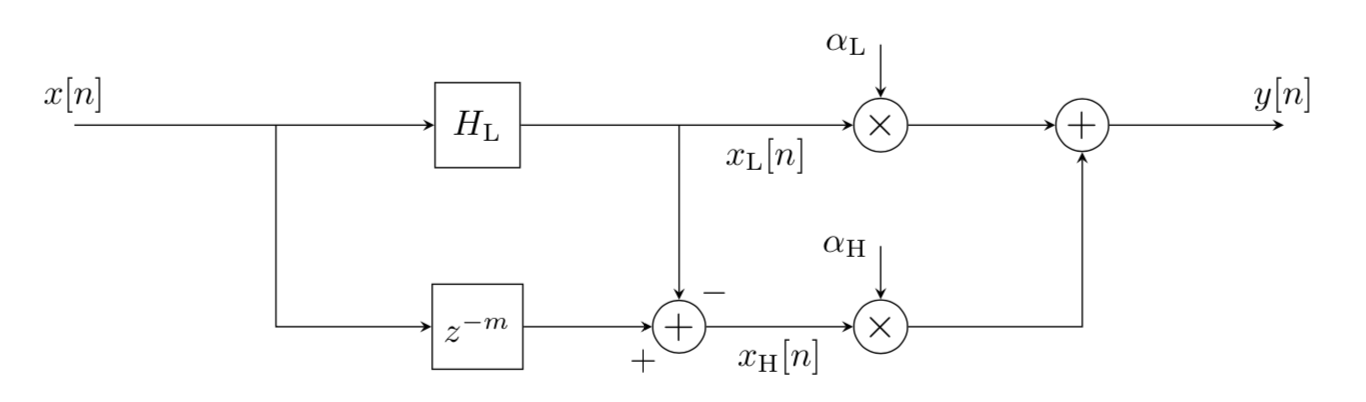
\includegraphics[scale = 0.5]{structure}
\caption{Structure of the equalizer [1]}
\label{fig:structure}
\end{figure}

The structure of the equalizer is shown above. The component $H_L$ represents a low-pass filter that filters out the low-frequencies in $x[n]$ and gives $x_L[n]$. The signal $x_H[n]$ represents $x[n]$ that has been passed through a high-pass filter. 

We introduce the components $\alpha_L$ and $\alpha_H$ to control the amount of low or high-frequencies in the output signal.
\begin{equation}
	y[n] = \alpha_H x_H[n] + \alpha_L x_L[n]
\end{equation}

The equalizer must allow the user to recover the input signal (with a possible delay) when we use all the frequencies present in $x[n]$ ($\alpha_H = \alpha_L = 1$) independently from the low-pass filter $H_L$.
\newline

$y[n] = \alpha_H x_H[n] + \alpha_L x_L[n]$

$\Leftrightarrow y[n] = \alpha_H (x[n-m] - x_L[n]) + \alpha_L x_L[n]$

$\Leftrightarrow y[n] = \alpha_H x[n-m] + (\alpha_L - \alpha_H)x_L[n]$

$\Leftrightarrow y[n] = \alpha_H x[n-m] + (\alpha_L - \alpha_H)(h_L*x)[n]$
\newline

\begin{equation}
	y[n] = x[n-m] \quad; \alpha_H = \alpha_L = 1
\end{equation}

So if $\alpha_H = \alpha_L = 1$, we have $y[n] = x[n-m]$,  $\forall$  $h_L$. The structure of the equalizer is in line with our expectations.


\section{Filters design}
\label{sec:filters design}

The filters are important components in an equalizer. The two basic filters are the low-pass and high-pass filter. In this section, we will design the filters such that the filters are Type I FIR filters and their lengths are under 55 taps.

\subsection{Low-pass filter}
The requirements for the low-pass filter are (in addition to those mentioned above) :
\begin{itemize}
	\item The normalized cutoff frequency is $\nu_c = \frac{1}{16}$.
	\item A suppression of at least $40 dB$ for all normalized frequencies above $\nu = \frac{1}{8}$.
\end{itemize}

\begin{figure}[!ht]
\centering
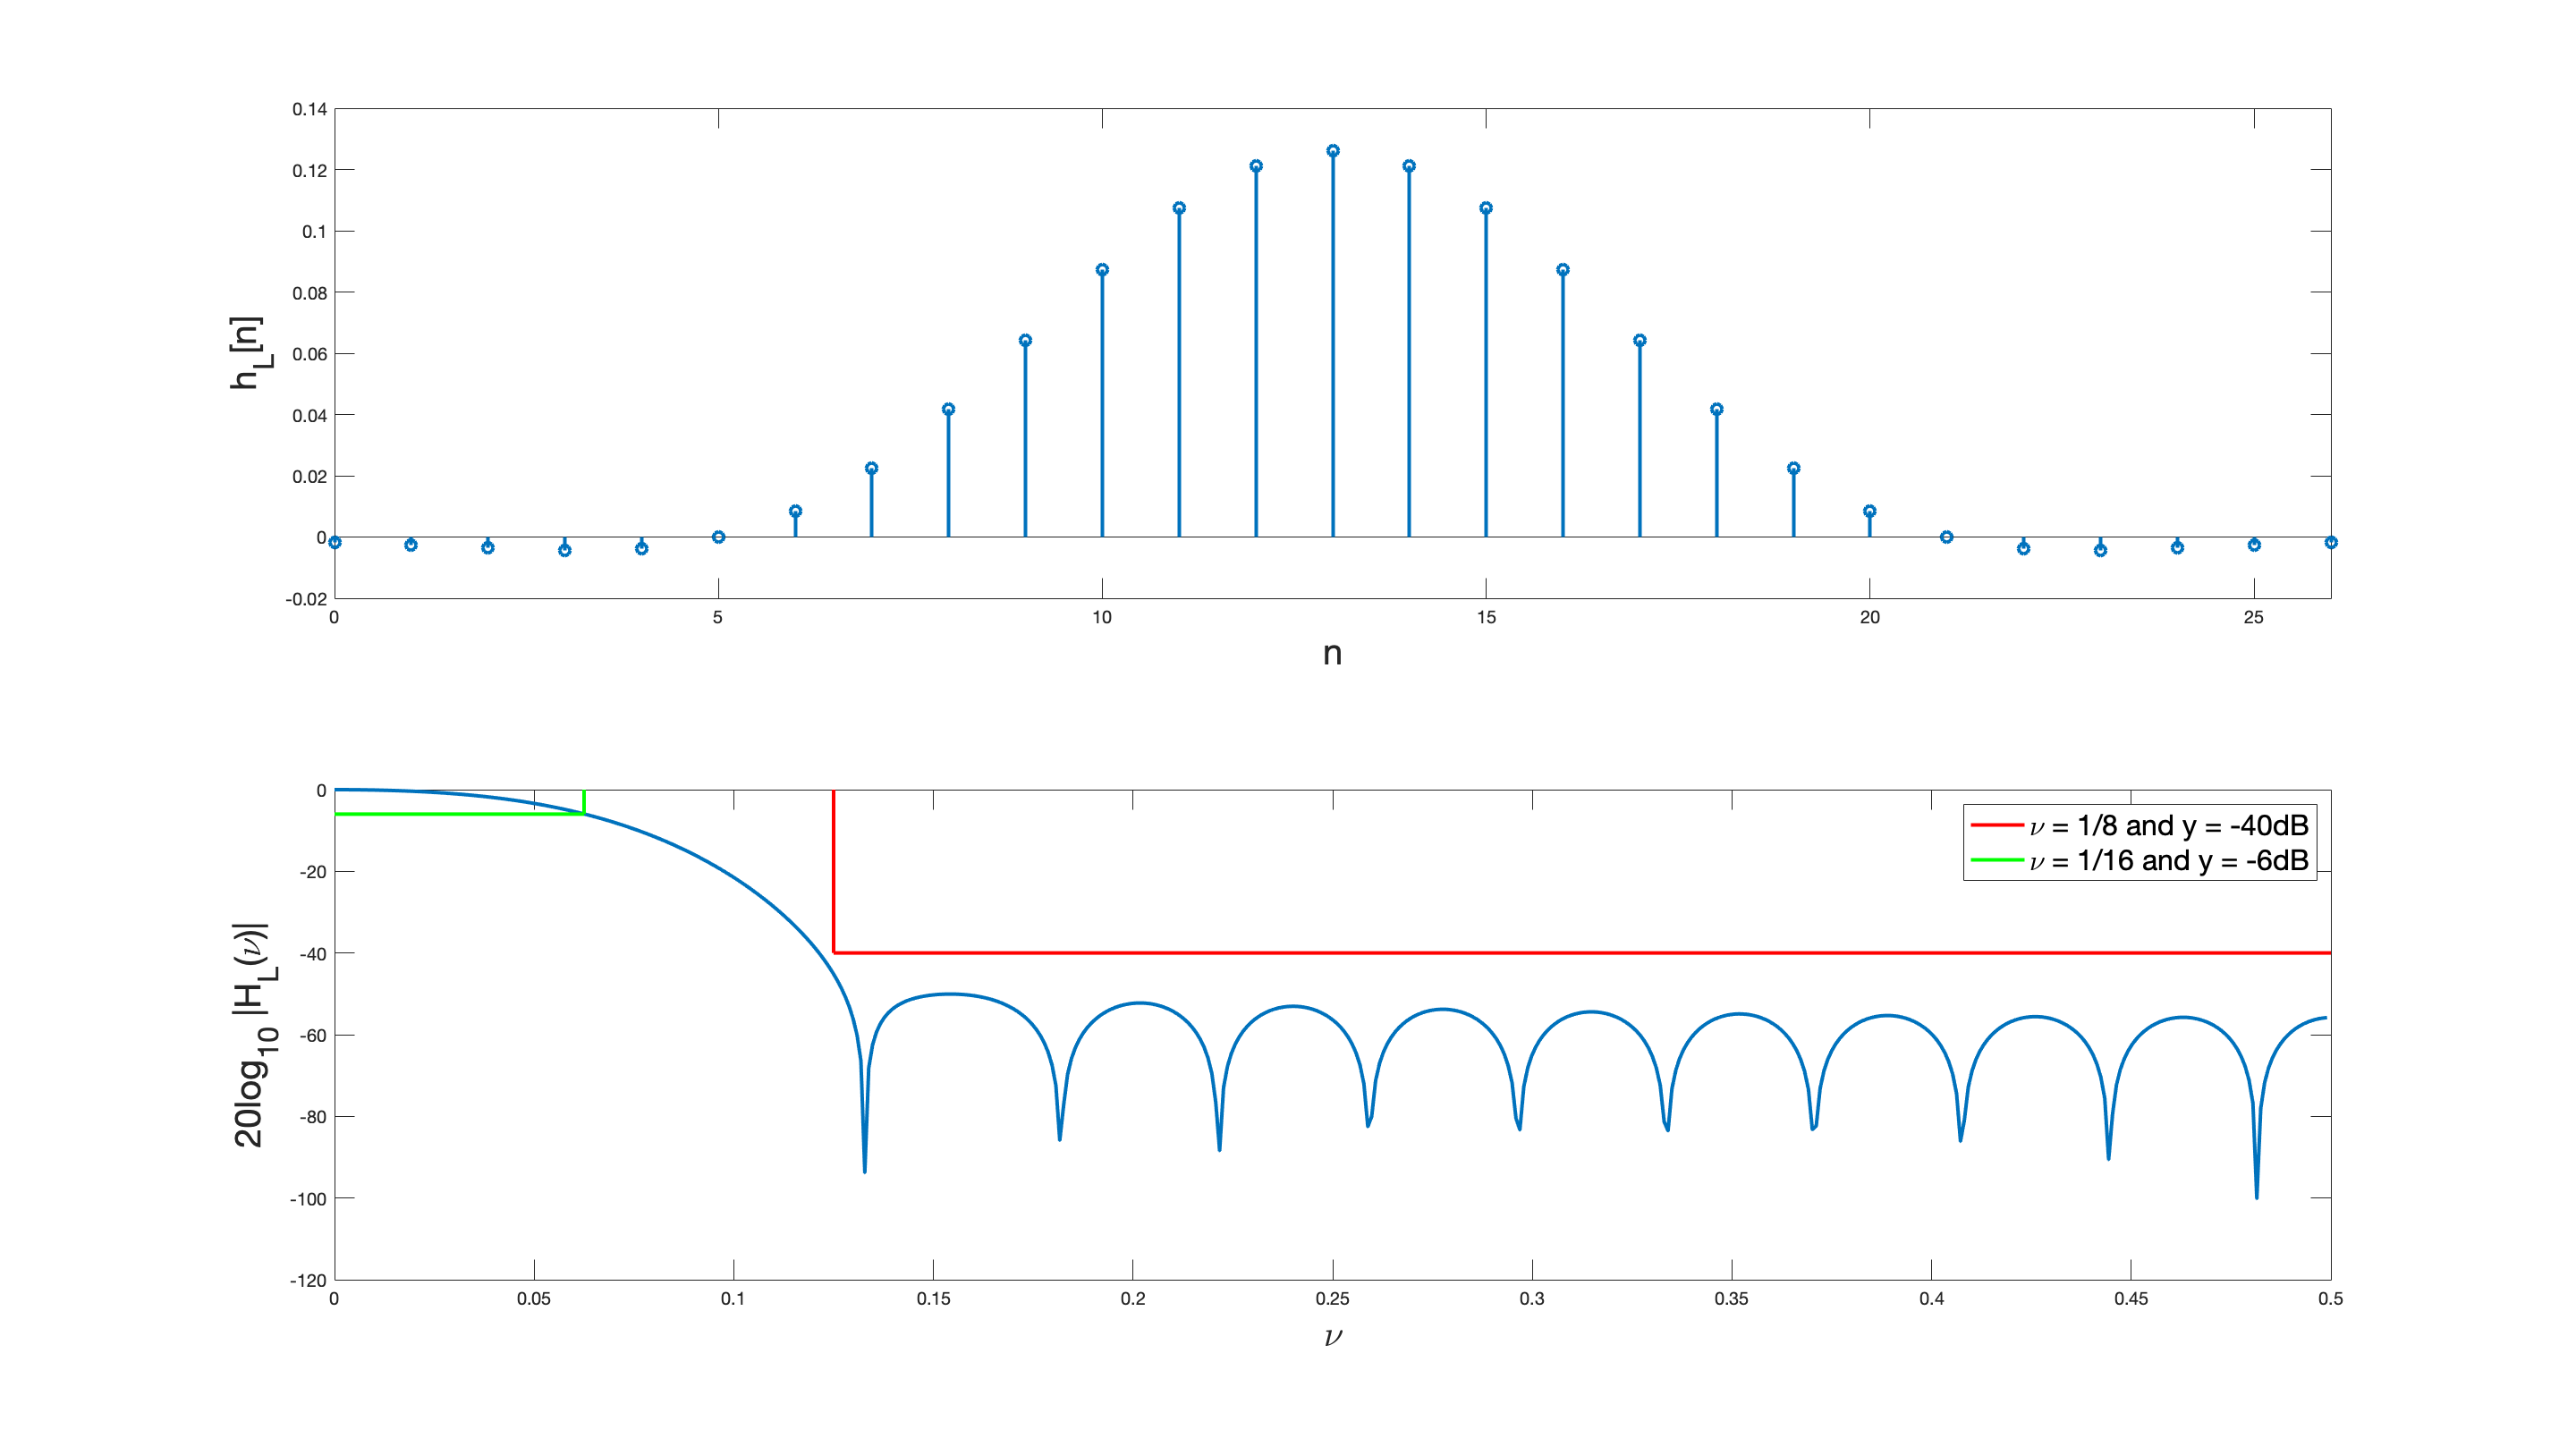
\includegraphics[scale = 0.12]{lowpass}
\caption{Low-pass filter, filter order M = 26}
\label{fig:lowpass}
\end{figure}

To generate the filter above, I used a windowing method. The windowing method consists in cutting an ideal filter impulse with a window.

To know which window to use, we have to look at the requirements for the filter. From the requirements about the frequencies, we can deduce that the filter must have small side-lobes and a main lobe not too large to respect the specification about attenuation. Thus the Hamming or the Hanning window seems to be a good choice.

The minimal filter order that respects the requirements with a Hamming window is M = 25. We know that the filter is a Type I filter so the filter order M must be even. Thus, I have chosen a filter order M = 26.

\subsection{High-pass filter}

From the structure of the equalizer we have the following equation : 
\begin{equation}
	x_H[n] = x[n-m] - x_L[n] = (x*h_H)[n] \Leftrightarrow h_H[n] = \delta[n-m] - h_L[n]
\end{equation}

We want $h_H[n]$ to be a Type I high-pass filter, so we know that M must be even and the filter must be symmetric around $\frac{M}{2}$. The only $m$ that respects these conditions is $m = \frac{M}{2}$.

\begin{figure}[!ht]
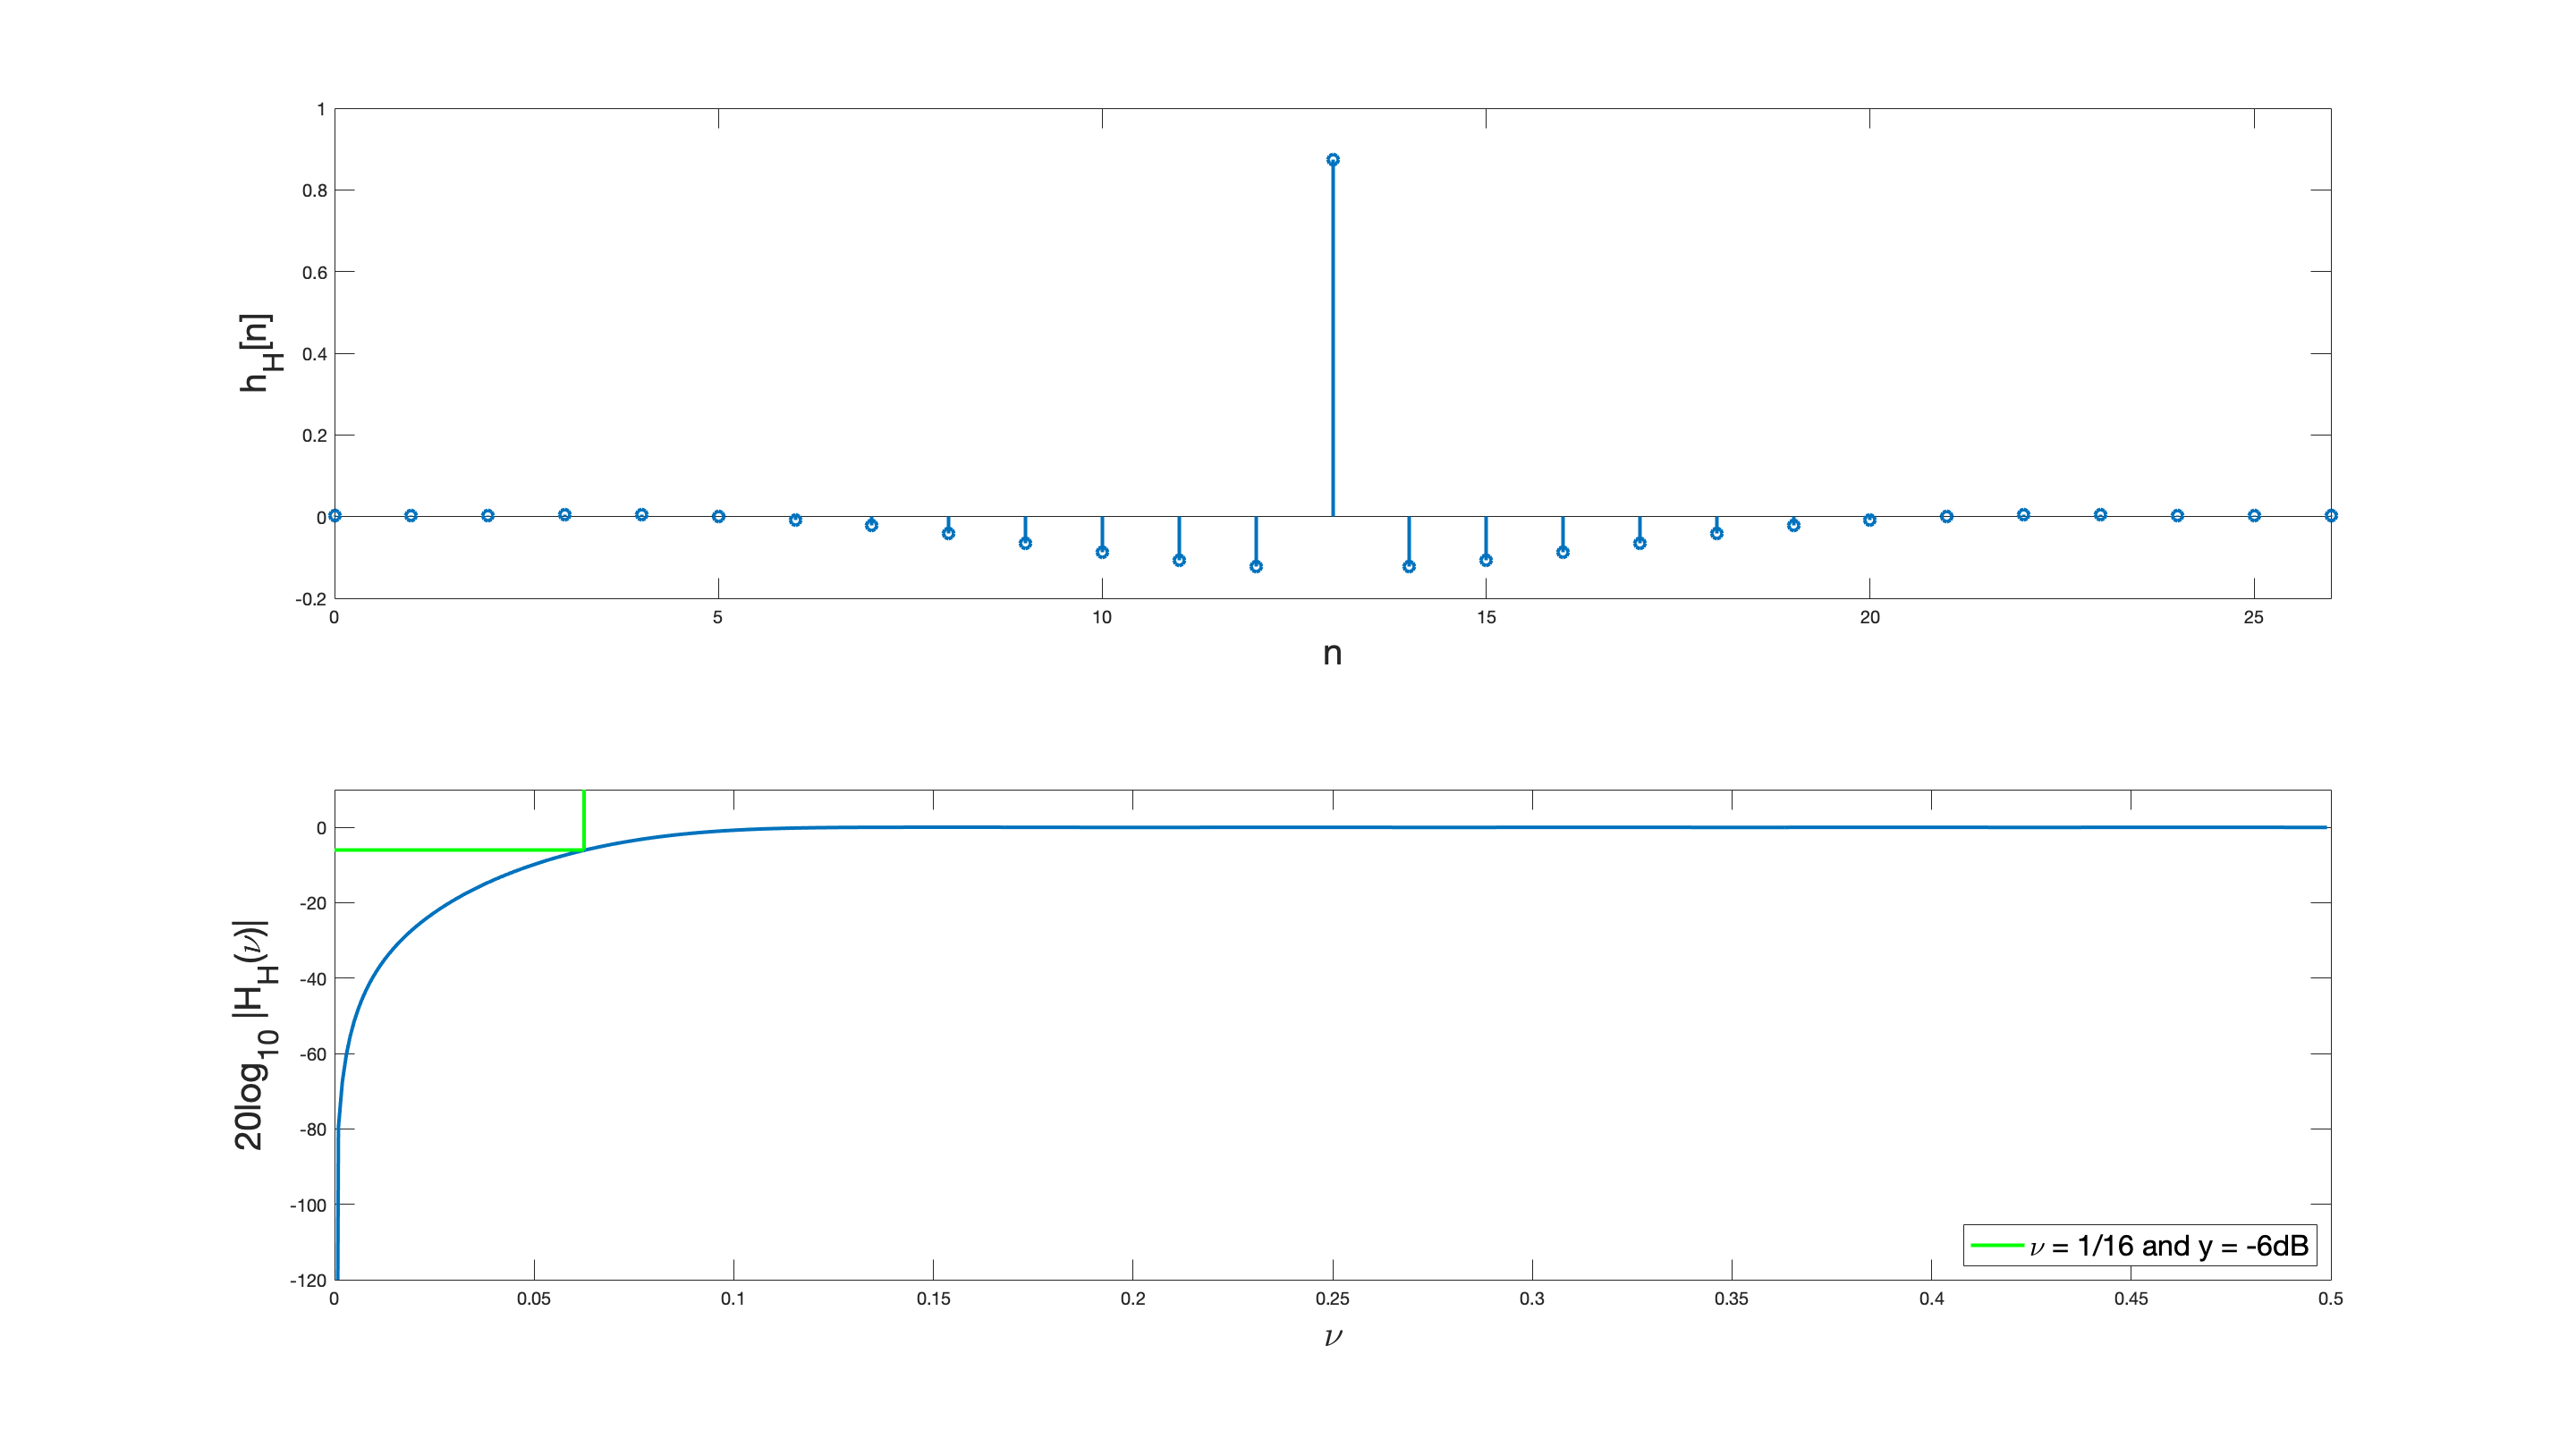
\includegraphics[scale = 0.12]{highpass}
\caption{High-pass filter, filter order M = 26}
\label{fig:high}
\end{figure}

We can see from the figure above that this high-pass filter respects the criteria to be a Type I FIR filter : 

\begin{itemize}
	\item[] $\rightarrow$ $h_H[n]$ is a filter with an even order $M = 26$
	\item[] $\rightarrow$ $h_H[n]$ is symmetric around $\frac{M}{2}$
\end{itemize}


\section{Fixed Point filter}
\label{sec:fixed Point filter}

On the platform, the filter will be quantized due to the fixed-point processing so, in this part,  we will study the influence of the quantization on the filter. we will only focus on the low-pass filter.

\subsection{Quantized low-pass filter}

The quantized low-pass filter is implemented by $h[n] = 2^{-F} [2^{F}h_L[n]]$ where $F$ is the number of bits to implement the filter ($ 0 < F \leq 16$) and $[.]$ the rounding operation.
\newline

From the figure bellow we can see that with 10 bits to quantized the filter, we still respect the requirements. 

\newpage

\begin{figure}[!ht]
\centering
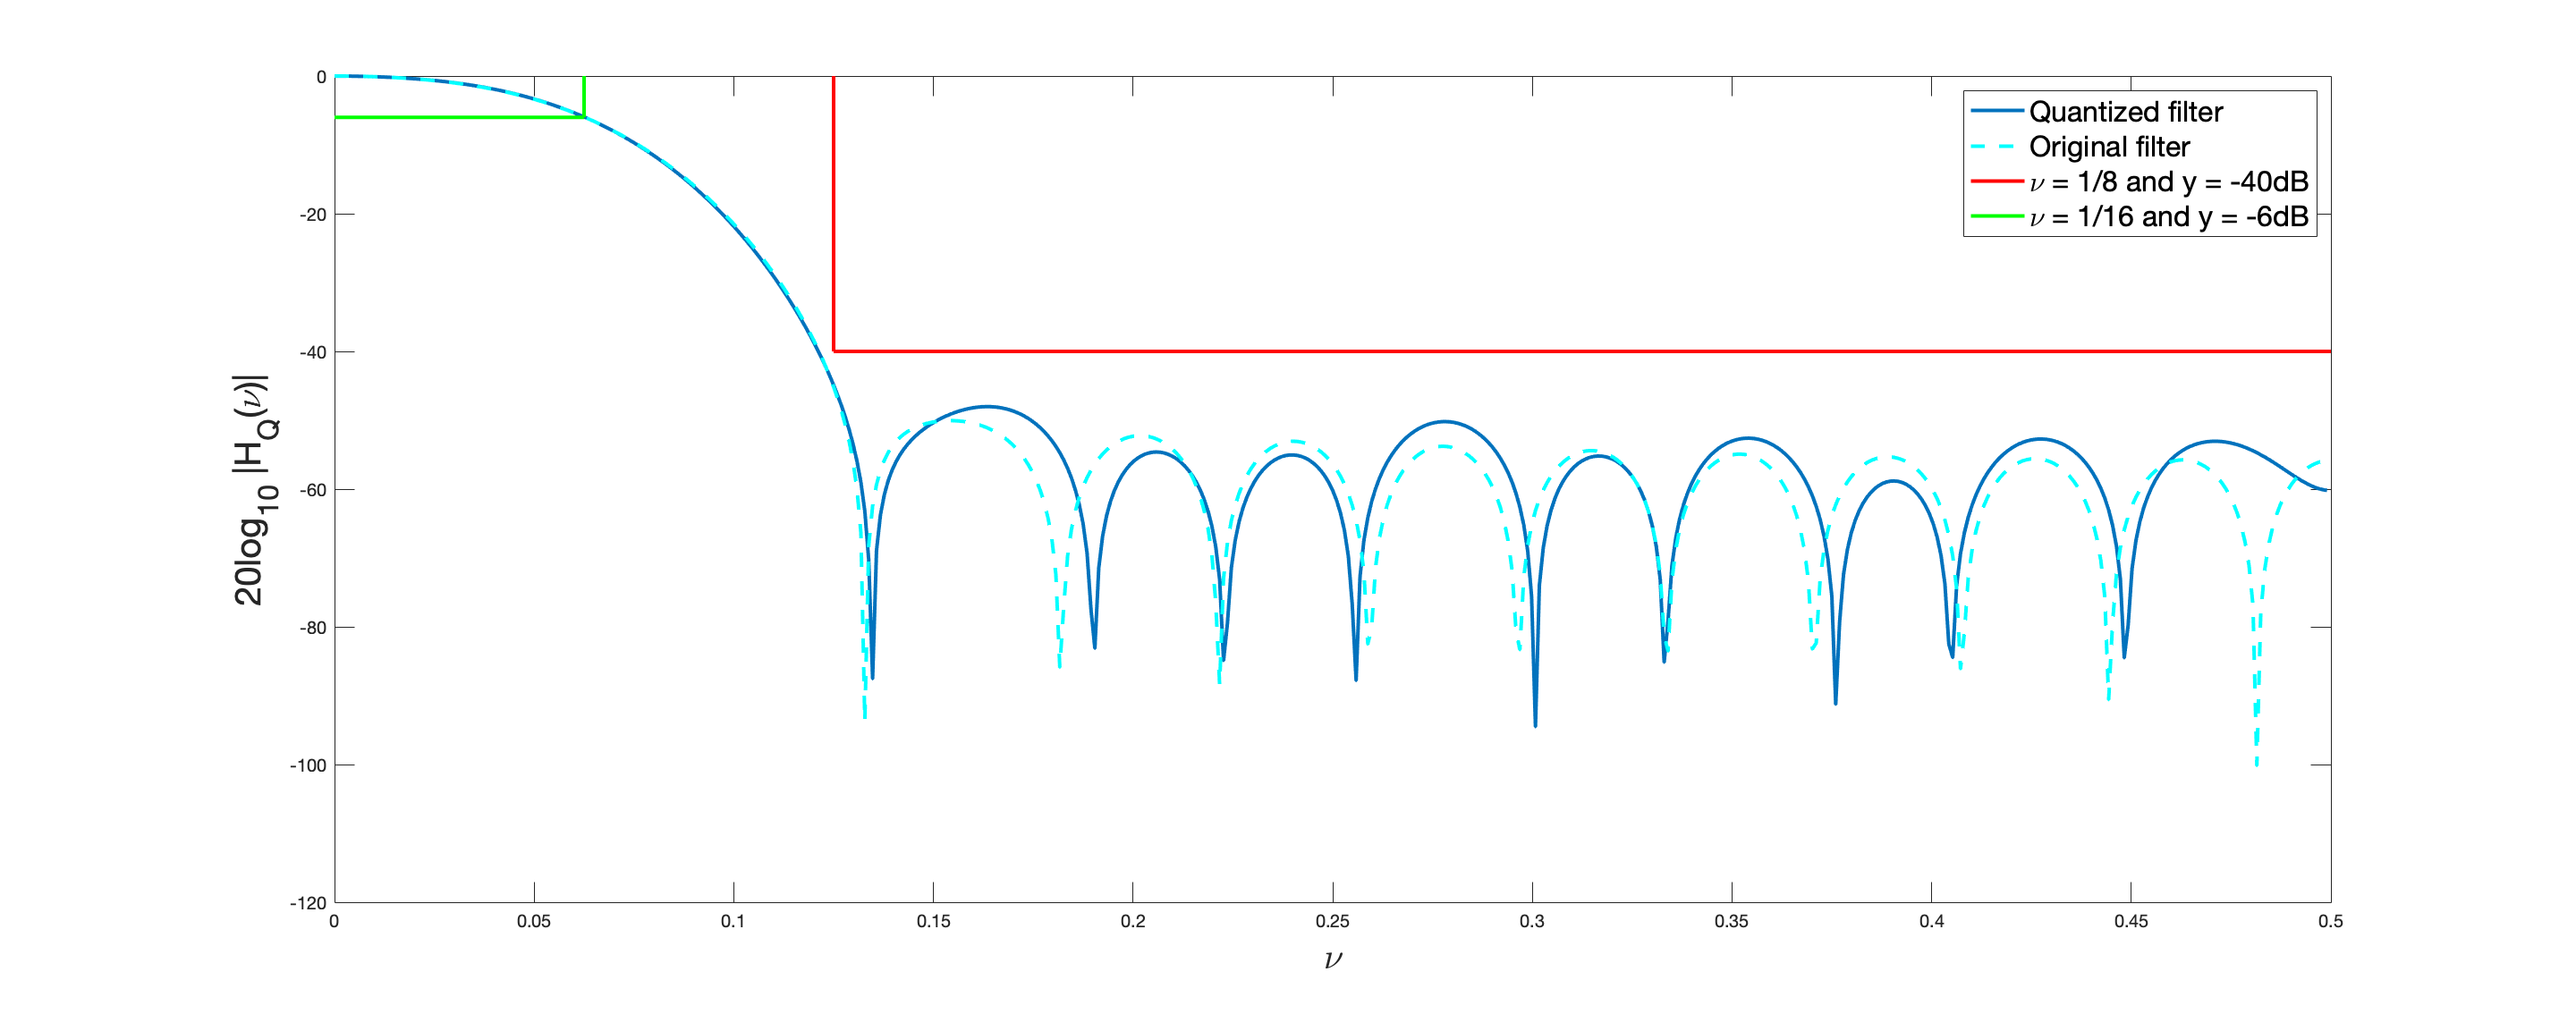
\includegraphics[scale = 0.12]{fpf}
\caption{Low-pass fixed point filter with F = 10 bits and compared to the original filter}
\label{fig:fpf}
\end{figure}


In order to find the number of bits needed to respect the specifications, I used the trials and errors method to calculate the DTFT of the quantized filter and verified if the requirements were respected. We can observe the more bits we use, the better the filter is approximated and I took the minimal number of bits needed to respects the requirements of the filter.


\subsection{Quality of the measure}
In order to quantified the quality of the measure we will estimate the SQNR.
\begin{equation}
	SQNR = \frac{E[x_L[n]^2]}{E[(x_L[n] - x_Q[n])^2]}
\end{equation}


The SQNR has been estimated by following these steps :

\begin{itemize}
	\item Generate a large uniform sequence of integer $x[n]$ in the range $[-2^{11}; 2^{11}]$
	\item Filter $x[n]$ with $h_L[n]$ and $h_Q[n]$ to obtain $x_L[n]$ and $x_Q[n]$
	\item Estimate the statistics of $x_L[n]$ and $x_L[n] - x_Q[n]$ (mean and variance)
	\item Estimate the SQNR
\end{itemize}

With $F = 10$, we obtain $SQNR = 47dB$. The SQNR can be increased by using more bits but only a subjective experience of the audio will say if the quality of the measure is enough or not.

\section{Conclusions}
\label{sec:conclusions}
We have seen in this project how to design a Type I FIR filter (a low-pass filter) by using a windowing method. The other filter (the high-pass filter) was deduced using the structure of the equalizer.

The platform does not have a floating point unit so we designed the filter by simulating a fixed point processing and chose a proper number of bits that approximate the filters and respect the requirements. However, a listening is required to confirm that this number of bits is enough.



\begin{thebibliography}{99}
\bibitem{latexmanual} \textsl{Project Assignment, HT 2018, EQ2300 Digital Signal Processing}
\end{thebibliography}
\end{document}
